\chapter{Diseño del sistema}
	
	En este capítulo se detallarán los módulos que serán necesarios utilizar e implementar. Para cada módulo se especificará el nombre del módulo, una descripción general del módulo, las variables que usa y las funciones que utiliza. Estos módulos se extraen tanto de los diagramas de casos de uso y de los diagramas de secuencia como de la propia definición del problema. En cada uno de los módulos que se describirán a continuación se distinguirán principalmente los siguiente apartados:
	
	\begin{itemize}
		\item \textit{Nombre del módulo:} se especificará el nombre del módulo que se vaya a explicar. Este nombre será identificativo y se corresponderá con el estilo que tiene el toolbox nnet de Matlab para que la integración sea lo más correcta posible.
		\item \textit{Descripción general del módulo:} se hará una descripción general de la funcionalidad y el manejo que tendrá el módulo.
		\item \textit{Funciones del módulo:} en el caso de que el módulo en sí no sea una función, se detallarán las funciones que se usan para el correcto funcionamiento de dicho módulo.
	\end{itemize}
	
	\section{Diseño de los módulos}
	
		En esta sección se va a realizar la especificación de los módulos que contendrá el sistema. Para ello, se hará uso de diagramas de paquetes y así poder ver la estructuración del sistema.\\
		
		En el Lenguaje Unificado de Modelado, los diagramas de Paquetes se usan para reflejar la organización de paquetes y sus elementos. Los usos más comunes de para los diagrama de paquete son para organizar diagramas de casos de uso y diagramas de clases, estos paquetes son como grandes contenedores de clases.	Los elementos contenidos en un paquete comparten el mismo espacio de nombres, esto significa que los elementos contenidos en un mismo espacio de nombres específico deben tener nombres únicos. Como otra característica de estos diagramas, cada paquete se debe identificar con un nombre único y opcionalmente mostrar todos los elementos dentro del mismo.\\
		
		Antes de realizar la especificación de cada módulo por separado, en la Figura \ref{fig:paquetes0} se muestra la estructuración general del sistema diseñado para que se ajuste lo más posible y con una estructura similar al toolbox nnet de Matlab.
		
		\begin{figure}[h]
			\centering
			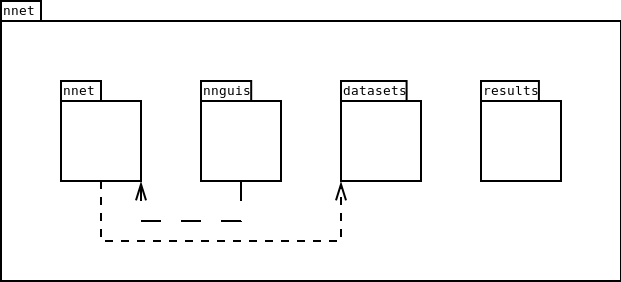
\includegraphics[scale=0.6]{uml/DiagramaPaquetes0.png}
			\caption{Diagrama de Paquetes principal}
			\label{fig:paquetes0}
		\end{figure}
		
		\subsection{Módulo principal nnet}
		
			Este será el módulo principal del sistema el cual contendrá los submódulos necesarios para el funcionamiento del sistema. Cada submódulo contendrá las funciones necesarias para la creación y tratamiento de la red neuronal artificial junto con el algoritmo propuesto en este proyecto. La organización de este módulo contiene una estructura similar al del toolbox nnet de Matlab.\\
			
			La Figura \ref{fig:paquetes1} muestra el diagrama de Paquetes para este módulo.
			
			\begin{figure}[h]
				\centering
				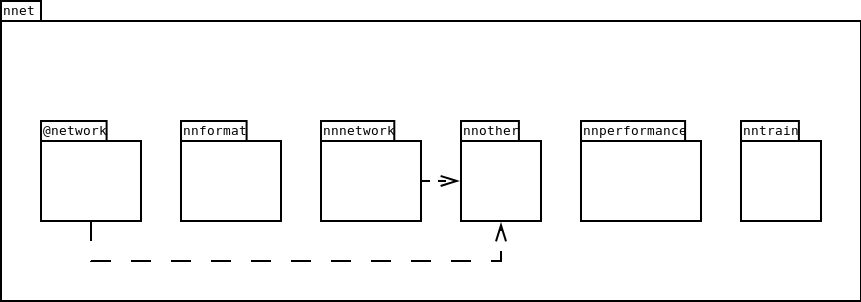
\includegraphics[scale=0.5]{uml/DiagramaPaquetes1.png}
				\caption{Diagrama de Paquetes del módulo nnet diseñado}
				\label{fig:paquetes1}
			\end{figure}
			
			La Tabla \ref{modulo_nnet} muestra la especificación breve del módulo principal.
			
			\begin{table}[!h]
				\centering
				\begin{tabular}{l|p{.5\linewidth}}
					\hline Nombre & nnet \\ 
					\hline Descripción & Módulo principal del sistema. Contendrá los principales submódulos para que el sistema funcione. \\ 
					\hline 
				\end{tabular}
				\caption{Especificación módulo nnet}
				\label{modulo_nnet}
			\end{table}
		
			\subsubsection{Módulo @network}
			
			La Tabla \ref{modulo_@network} muestra la especificación detallada del módulo así como la descripción de las funciones que contiene.
			
			\begin{table}[!h]
				\centering
				\begin{tabular}{l|p{.5\linewidth}}
					\hline Nombre & @network \\ 
					\hline Descripción & Módulo que contiene las funciones para el entrenamiento y simulación de la red neuronal pero ajustada para que los métodos se basen en la ordinalidad. \\ 
					\hline Funciones & \textit{OSIM}: función para simular una red neuronal ordinal a partir de los datos de entrada del conjunto de datos seleccionado y que devolverá las salidas obtenidas.
					
					\textit{OTRAIN}: función para entrenar una red neuronal ordinal a partir de los datos de entrada y los datos objetivo del conjunto de datos seleccionado. El entrenamiento se producirá haciendo uso del algoritmo propuesto en este proyecto, es decir, ORNnet. \\ 
					\hline 
				\end{tabular}
				\caption{Especificación módulo @network}
				\label{modulo_@network}
			\end{table}
			
			\subsubsection{Módulo nnformat}
		
			La Tabla \ref{modulo_nnformat} muestra la especificación detallada del módulo así como la descripción de las funciones que contiene.
			
			\begin{table}[!h]
				\centering
				\begin{tabular}{l|p{.5\linewidth}}
					\hline Nombre & nnformat \\ 
					\hline Descripción & Módulo que contiene la función para realizar una división estratificada de los datos. \\ 
					\hline Funciones & \textit{DIVIDESTRA}: función que realiza una división estratificada de los datos a partir de los datos objetivos los cuales son tratados para obtener un vector de elementos con identificación a la clase a la que pertenecen. \\ 
					\hline 
				\end{tabular}
				\caption{Especificación módulo nnformat}
				\label{modulo_nnformat}
			\end{table}
			
			\subsubsection{Módulo nnnetwork}
		
			La Tabla \ref{modulo_nnnetwork} muestra la especificación detallada del módulo así como la descripción de las funciones que contiene.
			
			\begin{table}[!h]
				\centering
				\begin{tabular}{l|p{.5\linewidth}}
					\hline Nombre & nnnetwork \\ 
					\hline Descripción & Módulo que contiene la función necesaria para crear una red neuronal ordinal. \\ 
					\hline Funciones & \textit{NEWOFF}: función que crea una red neuronal ordinal a partir de los datos de entrada y objetivo del conjunto de datos seleccionado, por defecto habrá al menos dos capas ocultas donde la última capa oculta tendrá solamente una neurona sin bias y se usará como función de transferencia linear. La capa de salida tendrá por defecto como función de transferencia una sigmoide logarítmica. La función de entrenamiento especificada por defecto será la de entrenamiento basado en el algoritmo modificado iRProp+ ajustado para la implementación ordinal (ORNnet). Por último, la función por defecto para análisis será la del Error Cuadrado Medio (MSE) y se utilizará una división estratificada de los datos para la simulación de la red. \\ 
					\hline 
				\end{tabular}
				\caption{Especificación módulo nnnetwork}
				\label{modulo_nnnetwork}
			\end{table}
			
			\subsubsection{Módulo nnother}
			
			La Tabla \ref{modulo_nnother} muestra la especificación detallada del módulo así como la descripción de las funciones que contiene.
			
			\begin{table}[!h]
				\centering
				\begin{tabular}{l|p{.5\linewidth}}
					\hline Nombre & nnother \\ 
					\hline Descripción & Módulo que contiene las funciones auxiliares para carga de ficheros, realización de pre o post procesamiento de los conjuntos de datos de entrada u objetivos para convertirlos o transformarlos en conjuntos de datos válidos para su posterior tratado o realización de una división estratificada. \\ 
					\hline Funciones & \textit{CONVDATA}: función que realiza, a partir del conjunto de datos de entrada y de objetivos con el formato proporcionado por NNEP de la librería del grupo AYRNA, JCLEC, la creación de los nuevos conjuntos de datos compatibles para el tratado por Matlab.
					
					\textit{CONVOUTPUTS}: función que realiza el tratado del conjunto de datos de salida proporcionado por la simulación de la red neuronal ordinal convirtiéndolo en un conjunto de datos de salida válido para su posterior procesado.
					
					\textit{GETSTRA}: función que realiza, a partir de la transformación de un conjunto de datos objetivos, la creación del vector de elementos estratificados.
					
					\textit{IMPORTFILE}: función que realiza la carga de datos de un fichero a partir del nombre del fichero.
					
					\textit{KFOLD}: función que realiza una validación de cruce haciendo un k-Fold, que por defecto será de diez folds, a partir de los datos de entrada y objetivo de la red devolviendo el número óptimo de neuronas en la capa oculta.
					
					\textit{TRANSDATA}: función que realiza la transformación de los datos objetivos para obtener como resultado un nuevo conjunto de datos objetivos compatible para el procesamiento del MSE. \\ 
					\hline 
				\end{tabular}
				\caption{Especificación módulo nnother}
				\label{modulo_nnother}
			\end{table}
			
			\subsubsection{Módulo nnperformance}
			
			La Tabla \ref{modulo_nnperformance} muestra la especificación detallada del módulo así como la descripción de las funciones que contiene.
			
			\begin{table}[!h]
				\centering
				\begin{tabular}{l|p{.5\linewidth}}
					\hline Nombre & nnperformance \\ 
					\hline Descripción & Módulo que contiene las funciones para medición del rendimiento de las salidas proporcionadas al entrenar y simular la red neuronal ordinal. \\ 
					\hline Funciones & \textit{CCRCALC}: función que realiza el cálculo del rango correctamente clasificado a partir de la matriz de confusión resultante de los datos de salida proporcionados al simular la red neuronal ordinal..
					
					\textit{MAECALC}: función que realiza el cálculo de error medio absoluto a partir de la matriz de confusión resultante de los datos de salida proporcionados al simular la red neuronal ordinal. \\ 
					\hline 
				\end{tabular}
				\caption{Especificación módulo nnperformance}
				\label{modulo_nnperformance}
			\end{table}
			
			\subsubsection{Módulo nntrain}
			
			La Tabla \ref{modulo_nntrain} muestra la especificación detallada del módulo así como la descripción de las funciones que contiene.
			
			\begin{table}[!h]
				\centering
				\begin{tabular}{l|p{.5\linewidth}}
					\hline Nombre & nntrain \\ 
					\hline Descripción & Módulo que contiene las funciones de entrenamiento para una red neuronal. Para una red neuronal ordinal se ha implementado la función de entrenamiento iRProp+ modificado con las especificaciones del algoritmo ORNnet. \\ 
					\hline Funciones & \textit{TRAINIRP}: función que realiza el entrenamiento de una red neuronal artificial aplicando el algoritmo iRProp+.
					
					\textit{TRAINIRPO}: función que realiza el entrenamiento de una red neuronal ordinal aplicando el algoritmo modificado iRProp+ con las modificación necesarias y especificadas por ORNnet. \\ 
					\hline 
				\end{tabular}
				\caption{Especificación módulo nntrain}
				\label{modulo_nntrain}
			\end{table}
			
	\section{Diseño de la interfaz}
		
		En esta sección se va a especificar cómo será el entorno que el usuario perciba al poner en funcionamiento la aplicación. Para ello se va a hacer uso de herramientas de prototipado de interfaces, concretamente de la herramienta web Balsamiq. En cada uno de los prototipos de la interfaz se especificarán cada uno de los elementos que contiene detalladamente.
		
		\subsection{Interfaz principal}
			
			La \textit{Interfaz principal} poseerá una estructura como la que se puede apreciar en la Figura \ref{fig:int0}.\\
			
			\begin{figure}[htbp]
				\centering
				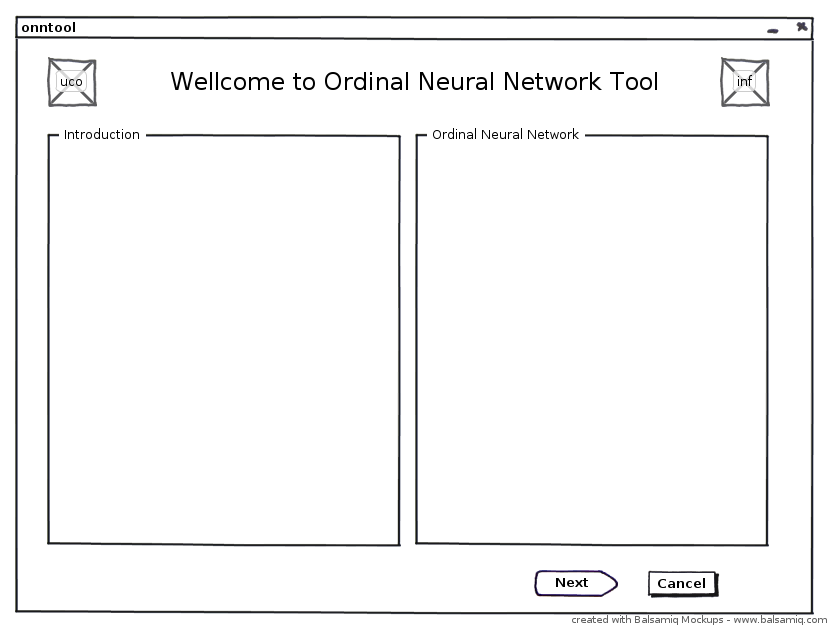
\includegraphics[scale=0.5]{interfaz/Interfaz_principal.png}
				\caption{Prototipo de la Interfaz principal}
				\label{fig:int0}
			\end{figure}
			
			La interfaz contendrá unas dimensiones de 800x600 píxeles en todo momento y, concretamente en ésta, los siguientes elementos ya sean interactivos o no:
			
			\begin{itemize}
				\item \textbf{Título:} contiene el título principal de bienvenida a la aplicación.
				\item \textbf{Imagen UCO:} imagen corporativa de la Universidad de Córdoba.
				\item \textbf{Imagen Informática:} imagen corporativa de los Ingenieros Informáticos.
				\item \textbf{Información Introducción:} cuadro que proporciona una breve información general sobre el uso de la aplicación.
				\item \textbf{Información Redes Neuronales Ordinales:} cuadro que proporciona una breve información sobre las redes neuronales artificiales ordinales.
				\item \textbf{Botón Siguiente:} botón que sirve para pasar a la siguiente interfaz.
				\item \textbf{Botón Cancelar:} botón que sirve para cerrar la interfaz en cualquier momento.
			\end{itemize}
			
			Los elementos comunes que aparezcan en las siguientes interfaces no se volverán a explicar para que no exista redundancia de información.
		
		\subsection{Interfaz de datos}
		
			La \textit{Interfaz de datos} poseerá una estructura como la que se puede apreciar en la Figura \ref{fig:int1}.\\
			
			\begin{figure}[htbp]
				\centering
				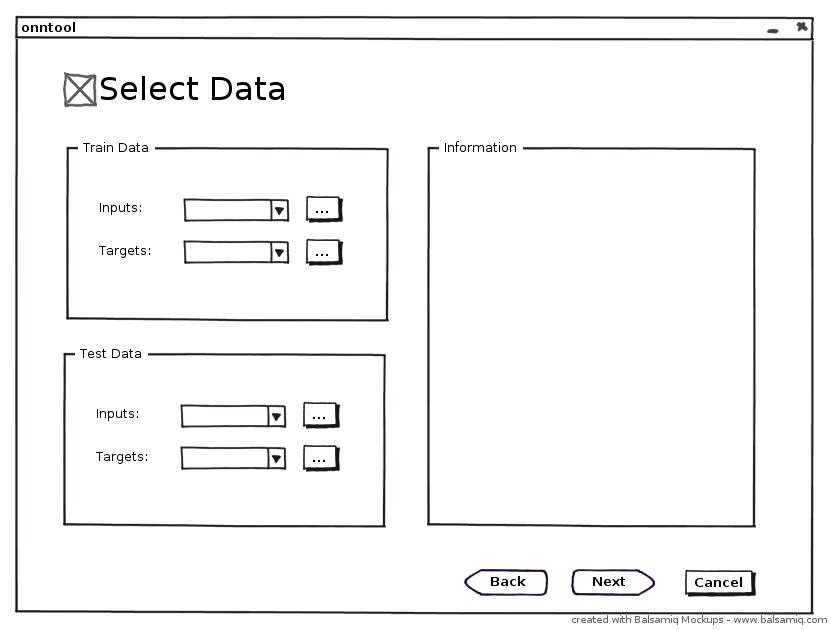
\includegraphics[scale=0.5]{interfaz/Interfaz_datos.png}
				\caption{Prototipo de la Interfaz de datos}
				\label{fig:int1}
			\end{figure}
			
			La interfaz contendrá los siguientes elementos, ya sean interactivos o no:
			
			\begin{itemize}
				\item \textbf{Título:} contiene el título representativo de la interfaz.
				\item \textbf{Botón de selección de datos de entrada (train y test):} botón que muestra la información del conjunto de datos de entrada.
				\item \textbf{Botón de selección de datos objetivos (train y test):} botón que muestra la información del conjunto de datos objetivos.
				\item \textbf{Botones de selección de datos (train y test):} botón que, a partir de una interfaz de carga de datos, selecciona un fichero externo y carga los datos para tratarlos.
				\item \textbf{Información de ayuda:} cuadro que proporciona una breve información de la interfaz.
				\item \textbf{Botón Atrás:} botón que sirve para pasar a la interfaz anterior.
			\end{itemize}
			
		\subsection{Interfaz para la creación de la red neuronal}
		
			La \textit{Interfaz de red neuronal} poseerá una estructura como la que se puede apreciar en la Figura \ref{fig:int2}.\\
			
			\begin{figure}[htbp]
				\centering
				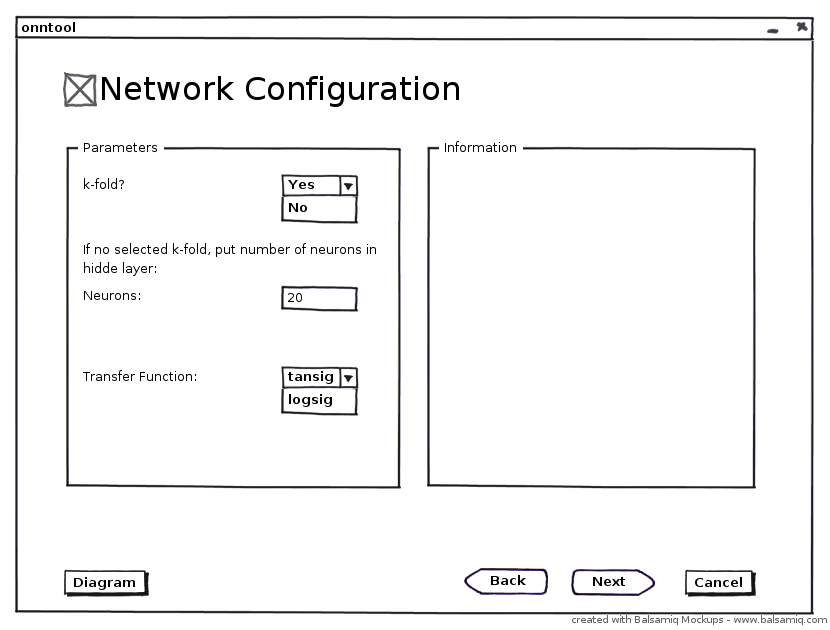
\includegraphics[scale=0.5]{interfaz/Interfaz_net.png}
				\caption{Prototipo de la Interfaz de red neuronal}
				\label{fig:int2}
			\end{figure}
			
			La interfaz contendrá los siguientes elementos, ya sean interactivos o no:
			
			\begin{itemize}
				\item \textbf{Opción de realización de k-fold:} botón que da la opción de realizar un k-fold para los conjuntos de datos.
				\item \textbf{Número de neuronas:} en caso de no activar la opción de k-fold se podrá especificar el número de neuronas que tendrá la capa oculta.
				\item \textbf{Opción para la función de transferencia:} al igual que el anterior, cuando no esté activa la opción del k-fold, se tendrá que especificar la función de transferencia.
				\item \textbf{Botón de Diagrama:} botón que da la posibilidad de mostrar de forma gráfica como se organiza la red neuronal artificial ordinal.
			\end{itemize}
			
		\subsection{Interfaz de entrenamiento y simulación}
		
			La \textit{Interfaz de entrenamiento y simulación} poseerá una estructura como la que se puede apreciar en la Figura \ref{fig:int3}.\\
			
			\begin{figure}[htbp]
				\centering
				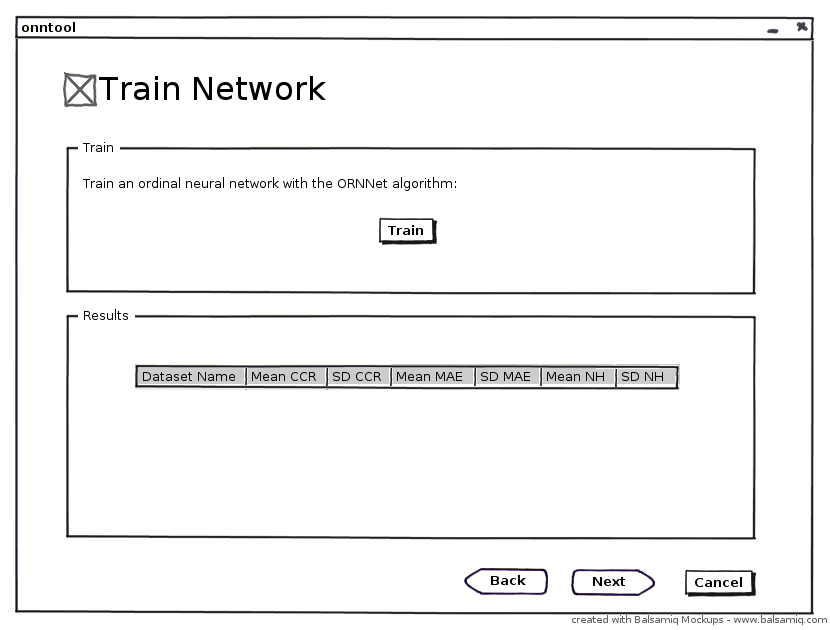
\includegraphics[scale=0.5]{interfaz/Interfaz_train.png}
				\caption{Prototipo de la Interfaz de entrenamiento}
				\label{fig:int3}
			\end{figure}
			
			La interfaz contendrá los siguientes elementos, ya sean interactivos o no:
			
			\begin{itemize}
				\item \textbf{Botón de entrenamiento:} botón que entrena y simula la red neuronal a partir de los datos de entrenamiento y test del conjunto de datos.
				\item \textbf{Resultados:} muestra los resultados obtenidos a partir de la simulación.
			\end{itemize}
		
		\subsection{Interfaz de exportación de datos}
		
			La \textit{Interfaz de exportación} poseerá una estructura como la que se puede apreciar en la Figura \ref{fig:int4}.\\
			
			\begin{figure}[htbp]
				\centering
				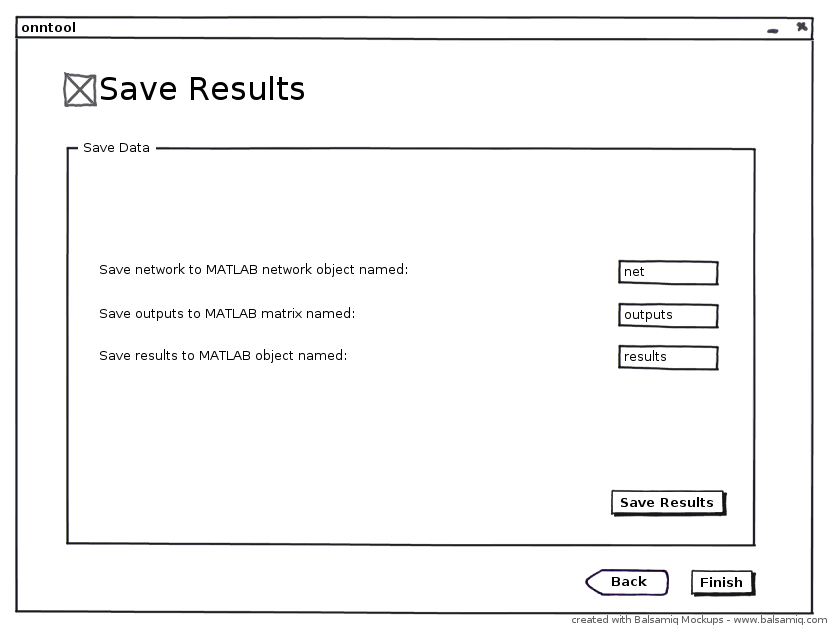
\includegraphics[scale=0.5]{interfaz/Interfaz_export.png}
				\caption{Prototipo de la Interfaz de exportación}
				\label{fig:int4}
			\end{figure}
			
			La interfaz contendrá los siguientes elementos, ya sean interactivos o no:
			
			\begin{itemize}
				\item \textbf{Nombre para guardar la red neuronal:} campo para especificar como se llamará la variable que almacenará la estructura de la red neuronal.
				\item \textbf{Nombre para guardar las salidas obtenidas:} campo para especificar como se llamará la variable que almacenará la matriz de salida.
				\item \textbf{Nombre para guardar los resultados de salida (CCR, MAE, NH):} campo para especificar como se llamará la variable que almacenará la matriz de resultados.
				\item \textbf{Botón Guardar Resultados:} botón que guardará los resultados en el espacio de trabajo de Matlab.
				\item \textbf{Botón Finalizar:} botón que cerrará la interfaz al dar el proceso por finalizado.
			\end{itemize}
